\begin{lstlisting}
Section 7.4:  3,  4,   5,  7,  8  
Section 7.5:  10,  11  
Section 7.6:  1,  2,  6, 9 (ed7: 1, 2, 5, 8)
\end{lstlisting}
\begin{exercise}
\begin{figure}[H]
\centering
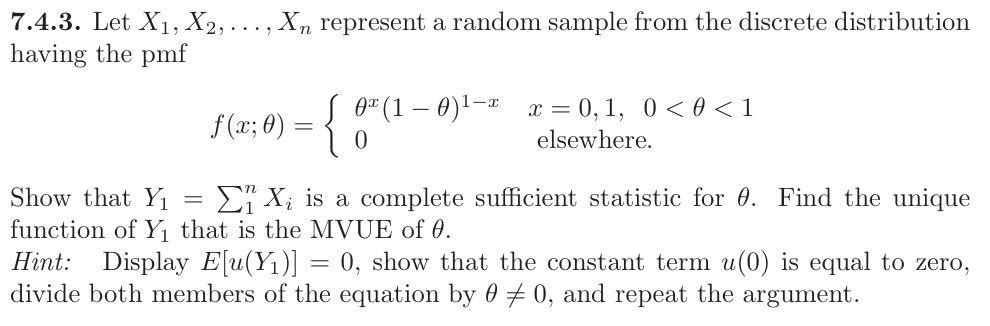
\includegraphics[width=\textwidth]{hw12-2025052716.png}
% \caption{}
\label{}
\end{figure}
\end{exercise}
\[
\frac{\prod_{i=1}^{n} f(x_i;\theta)}{f_{Y_1}\left( \sum x_i;\theta \right)}=\frac{\theta^{\sum x_i}(1-\theta)^{n-\sum x_i }}{\binom{n}{\sum x_i} \theta^{\sum x_i}(1-\theta)^{n-\sum x_i}}=\frac{1}{\binom{n}{\sum x_i} }
\]
is irrelevant to $\theta$, thus $Y_1$ is sufficient. For any $u$ defined on $\{ 0,\dots,n \}$, assume that $\mathbb{E}(u(Y_1))=0$, then
\[
\sum_{y=0}^{n} u(y) \cdot \binom{n}{y} \theta^{y}(1-\theta)^{n-y}=0
\]
Choose appropriate $\theta$ 's such that the vector $\{ \binom{n}{y}\theta^{y}(1-\theta)^{n-y} \}_{y=0}^{n}$ takes more than $n+1$ different values. Then we have a homogeneous linear system for $u(0), \dots, u(n)$ where the number of equations exceeds the number of unknowns. Therefore, the only solution is the trivial solution, i.e., $u(y) = 0$ for all $y = 0, \dots, n$. Therefore $Y_1$ is complete.

As $\mathbb{E}Y_1=n\theta$, $\mathbb{E}\left( \frac{Y_1}{n} \right)=\theta$, thus $\frac{Y_1}{n}$ is the MVUE of $\theta$.

\begin{exercise}
\begin{figure}[H]
\centering
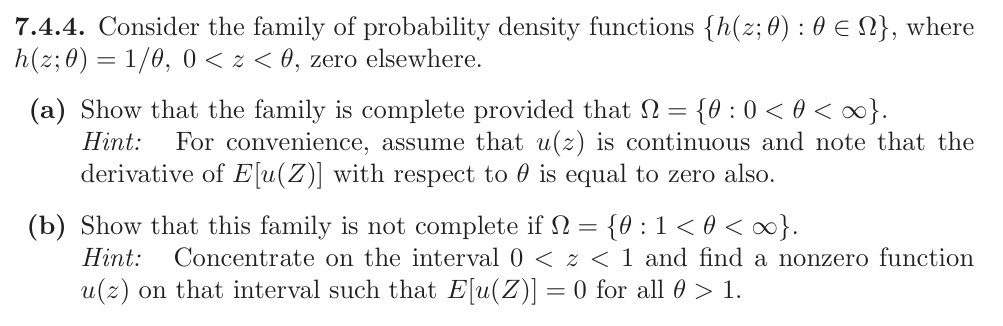
\includegraphics[width=\textwidth]{1-hw12-2025052716.png}
% \caption{}
\label{}
\end{figure}
\end{exercise}
A family of probability density functions $\{h(z;\theta):\theta\in\Omega\}$ is \textbf{complete} if for any measurable function $u(z)$ such that $\mathbb{E}[|u(Z)|] < \infty$, the condition $\mathbb{E}[u(Z)] = 0$ for all $\theta \in \Omega$ implies that $u(z) = 0$ almost everywhere for all $z$ in the support of the densities. For the given family $h(z;\theta) = 1/\theta$ for $0 < z < \theta$ (and zero elsewhere), the expectation is $\mathbb{E}[u(Z)] = \int_0^\theta u(z) \frac{1}{\theta} dz$.

(a) Completeness for $\Omega = \{\theta : 0 < \theta < \infty\}$

We want to show that if $\mathbb{E}[u(Z)] = 0$ for all $\theta \in (0, \infty)$, then $u(z) = 0$ almost everywhere for $z > 0$.

The condition $\mathbb{E}[u(Z)] = 0$ translates to:
\[
\int_0^\theta u(z) \frac{1}{\theta} dz = 0
\]
Since $\theta > 0$, we can multiply by $\theta$:
\[
\int_0^\theta u(z) dz = 0 \quad \text{for all } \theta \in (0, \infty)
\]
Let $G(\theta) = \int_0^\theta u(z) dz$. The condition states that $G(\theta) = 0$ for all $\theta > 0$.

Following the hint, if we assume $u(z)$ is continuous, then by the Fundamental Theorem of Calculus, the derivative of $G(\theta)$ with respect to $\theta$ is $u(\theta)$. Since $G(\theta)$ is identically zero for all $\theta > 0$, its derivative must also be zero:
\[
G'(\theta) = u(\theta) = 0 \quad \text{for all } \theta > 0
\]
Since $z$ is just a variable of integration, this implies $u(z) = 0$ for all $z > 0$.

More generally, without assuming continuity for $u(z)$ (we only need $u(z)$ to be integrable, which is required for $\mathbb{E}[u(Z)]$ to be defined), if $G(\theta) = \int_0^\theta u(z) dz = 0$ for all $\theta > 0$, then for any $0 < \theta_1 < \theta_2$:
\[
\int_{\theta_1}^{\theta_2} u(z) dz = \int_0^{\theta_2} u(z) dz - \int_0^{\theta_1} u(z) dz = G(\theta_2) - G(\theta_1) = 0 - 0 = 0
\]
This implies that $u(z) = 0$ almost everywhere on $(0, \infty)$. If $u(z)$ were non-zero on a set of positive Lebesgue measure, we could find an interval $(\theta_1, \theta_2)$ where the integral is non-zero, leading to a contradiction.

Thus, the family $\{h(z;\theta):\theta\in(0,\infty)\}$ is \textbf{complete}.

(b) Non-completeness for $\Omega = \{\theta : 1 < \theta < \infty\}$

We want to show that the family is not complete if $\Omega = \{\theta : 1 < \theta < \infty\}$. This means we need to find a function $u(z)$ that is not identically zero, for which $\mathbb{E}[u(Z)] = 0$ for all $\theta \in (1, \infty)$.

The condition $\mathbb{E}[u(Z)] = 0$ for all $\theta \in (1, \infty)$ implies:
\[
\int_0^\theta u(z) dz = 0 \quad \text{for all } \theta > 1
\]
Let $G(\theta) = \int_0^\theta u(z) dz$. Then $G(\theta) = 0$ for all $\theta > 1$.

This implies that $G'(\theta) = u(\theta) = 0$ almost everywhere for $\theta > 1$. So, any such $u(z)$ must be $0$ almost everywhere for $z > 1$.

For $u(z)$ to be a non-zero function overall, it must be non-zero for some $z \in (0, 1]$.
If $u(z) = 0$ for $z > 1$, then for any $\theta > 1$:
\[
\int_0^\theta u(z) dz = \int_0^1 u(z) dz + \int_1^\theta u(z) dz
\]
Since $u(z) = 0$ for $z > 1$, the second integral $\int_1^\theta u(z) dz = \int_1^\theta 0 dz = 0$.
So, the condition $\mathbb{E}[u(Z)]=0$ reduces to:
\[
\int_0^1 u(z) dz = 0
\]
We need to find a function $u(z)$ such that:

\begin{enumerate}
	\item $u(z)$ is not identically zero.
	\item $u(z) = 0$ for $z > 1$.
	\item $\int_0^1 u(z) dz = 0$.
\end{enumerate}

Consider the function defined as follows (following the hint to concentrate on $0 < z < 1$):
\[
u(z) = \begin{cases} 1 & \text{if } 0 < z \le 1/2 \\ -1 & \text{if } 1/2 < z \le 1 \\ 0 & \text{if } z > 1 \text{ (and for } z \le 0) \end{cases}
\]
This function $u(z)$ is clearly not identically zero (e.g., $u(0.25) = 1$).
Let's verify $\int_0^1 u(z) dz$:
\[
\int_0^1 u(z) dz = \int_0^{1/2} (1) dz + \int_{1/2}^1 (-1) dz = [z]_0^{1/2} + [-z]_{1/2}^1 = \left(\frac{1}{2} - 0\right) + \left(-1 - \left(-\frac{1}{2}\right)\right) = \frac{1}{2} - \frac{1}{2} = 0
\]
Now, for any $\theta > 1$:
\[
\mathbb{E}[u(Z)] = \frac{1}{\theta} \int_0^\theta u(z) dz = \frac{1}{\theta} \left( \int_0^1 u(z) dz + \int_1^\theta u(z) dz \right)
\]
Since $u(z) = 0$ for $z > 1$, $\int_1^\theta u(z) dz = 0$. And we've shown $\int_0^1 u(z) dz = 0$.
Therefore, for any $\theta > 1$:
\[
\mathbb{E}[u(Z)] = \frac{1}{\theta} (0 + 0) = 0
\]
Since we found a non-zero function $u(z)$ such that $\mathbb{E}[u(Z)] = 0$ for all $\theta \in (1, \infty)$, the family $\{h(z;\theta):\theta\in(1,\infty)\}$ is \textbf{not complete}.

\begin{exercise}
\begin{figure}[H]
\centering
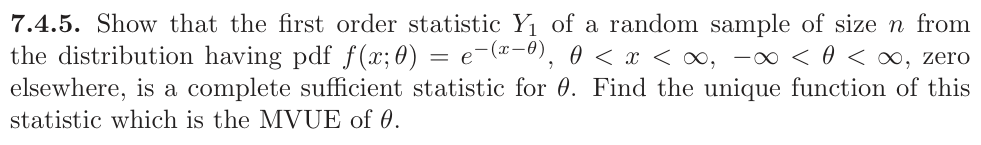
\includegraphics[width=\textwidth]{2-hw12-2025052716.png}
% \caption{}
\label{}
\end{figure}
\end{exercise}
\[
\begin{aligned}
f_{Y_1}(x) & =\frac{ \partial   }{ \partial x } \mathbb{P}(Y_1\leq x) \\
 & =\frac{ \partial   }{ \partial x } (1-\mathbb{P}(Y_1\geq x)) \\
 & =\frac{ \partial   }{ \partial x } (1-\mathbb{P}(X_i\geq x;\forall i)) \\
 & =\frac{ \partial   }{ \partial x } \left( 1-\prod_{i=1}^{n} \int_{x}^{+\infty} e^{ -(t-\theta) }\mathbb{1}_{x\geq \theta} \, \mathrm{d}t  \right) \\
 & =\frac{ \partial   }{ \partial x } (1-e^{ n(\theta-x) }\mathbb{1}_{x\geq \theta}) \\
 & =ne^{ n(\theta-x) }\mathbb{1}_{x\geq \theta}
\end{aligned}
\]
Then
\[
\frac{\prod_{i=1}^{n} f(x_i;\theta)}{f_{Y_1}(x_{(1)};\theta)}=\frac{\prod_{i=1}^{n} (e^{ -(x_i-\theta) }\mathbb{1}_{x_i\geq \theta})}{ne^{ n\theta -nx_{(1)}}\mathbb{1}_{x_{(1)\geq \theta}}}=\frac{1}{n}e^{ -\sum x_i +nx_{(1)}}
\]
is irrelenvant to $\theta$, where $x_{(1)}=\min_{i}x_i$. Thus $Y_1$ is sufficient. For any $u$, let
\[
g(\theta)\coloneqq \mathbb{E}(u(Y_1))=\int_{\theta}^{+\infty} u(y)ne^{ n\theta }e^{ -ny } \, \mathrm{d}y=0
\]
Then
\[
g'(\theta)=0\implies n\underbrace{ \int_{\theta}^{+\infty} u(y)ne^{ n\theta }e^{ -ny } \, \mathrm{d}y }_{ =0 } -u(\theta)n\underbrace{ e^{ n\theta }e^{ -n\theta } }_{ =1 }=0\implies u(\theta)=0
\]
Since $\theta$ is arbitrary, $u\equiv0$, thus $Y_1$ is complete.
\[
\mathbb{E}Y_1=\int_{\theta}^{+\infty} x\cdot ne^{ n(\theta-x) } \, \mathrm{d}x =\frac{n\theta  +1}{n}
\]
Then $Y_1-\frac{1}{n}$ is the MVUE of $\theta$.

\begin{exercise}
\begin{figure}[H]
\centering
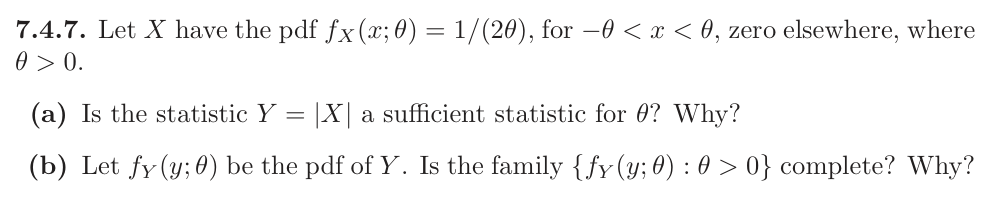
\includegraphics[width=\textwidth]{3-hw12-2025052716.png}
% \caption{}
\label{}
\end{figure}
\end{exercise}
\[
f_{Y}(x)=\frac{ \partial   }{ \partial x } \mathbb{P}(\lvert X \rvert \leq x)=\frac{ \partial   }{ \partial x } \mathbb{P}(-x\leq X\leq x)\mathbb{1}_{0\leq x<\theta}=\frac{ \partial   }{ \partial x } \int_{-x}^{x} 1/(2\theta) \, \mathrm{d}t \cdot \mathbb{1}_{0\leq x<\theta}=\frac{1}{\theta}\mathbb{1}_{0\leq x<\theta}
\]
\[
\frac{f_{X}(x;\theta)}{f_{Y}(\lvert x \rvert ;\theta)}=\frac{1/(2\theta)\mathbb{1}_{-\theta<x<\theta}}{1/\theta \cdot \mathbb{1}_{0\leq \lvert x \rvert <\theta}}=\frac{1}{2}
\]
Thus $Y$ is a sufficient statistic for $\theta$.
\[
\mathbb{E}[u(Y)]=\int_{0}^{\theta} u(y)\cdot\frac{1}{\theta} \, \mathrm{d}y=0\implies \int_{0}^{\theta} u(y) \, \mathrm{d}y=0,\quad \forall \theta>0
\]
For any $0 < \theta_1 < \theta_2$:
\[
\int_{\theta_1}^{\theta_2} u(z) dz = \int_0^{\theta_2} u(z) dz - \int_0^{\theta_1} u(z) dz = G(\theta_2) - G(\theta_1) = 0 - 0 = 0
\]
This implies that $u(z) = 0$ almost everywhere on $(0, \infty)$. If $u(z)$ were non-zero on a set of positive Lebesgue measure, we could find an interval $(\theta_1, \theta_2)$ where the integral is non-zero, leading to a contradiction.

Thus, the family $\{h(z;\theta):\theta\in(0,\infty)\}$ is \textbf{complete}.

\begin{exercise}
\begin{figure}[H]
\centering
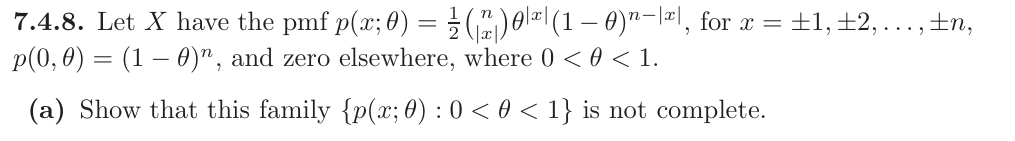
\includegraphics[width=\textwidth]{4-hw12-2025052716.png}
% \caption{}
\label{}
\end{figure}
\begin{figure}[H]
\centering
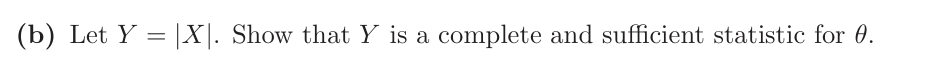
\includegraphics[width=\textwidth]{5-hw12-2025052716.png}
% \caption{}
\label{}
\end{figure}
\end{exercise}
(a)
Let
\[
\begin{aligned}
0 & =\mathbb{E}_{\theta}[g(X)] \\
 & =g(0)p(0;\theta)+\sum_{k=1}^{n} [g(k)p(k;\theta)+g(-k)p(-k;\theta)] \\
 & =g(0)(1-\theta)^{n}+\sum_{k=1}^{n} [g(k)+g(-k)]\binom{n}{k} \theta^{k}(1-\theta)^{n-k}\qquad \forall \theta\in(0,1)
\end{aligned}
\]
The above equality holds when $g(x)=x$. Then the family $\{ p(x;\theta):0<\theta<1 \}$ is not complete.

(b)
\[
p_{Y}(x;\theta)=p_{X}(-x;\theta)+p_{X}(x;\theta)=\binom{n}{x} \theta^{x}(1-\theta)^{n-x}\qquad x=0,1,\dots,n
\]
\[
\frac{p_{X}(x;\theta)}{p_{Y}(\lvert x \rvert ;\theta)}=\begin{cases}
\frac{1}{2} & x=\pm1,\pm2,\dots,\pm n \\
1 & x=0
\end{cases}
\]
Thus $Y$ is sufficient.
\[
\mathbb{E}(u(Y))=\sum_{k=0}^{n} u(k)\binom{n}{k} \theta^{k}(1-\theta)^{n-k}=0\qquad \forall \theta>0
\]
Then $u(k)=0$ for $k=0,1,\dots,n$. Thus $Y$ is complete.

\begin{exercise}
\begin{figure}[H]
\centering
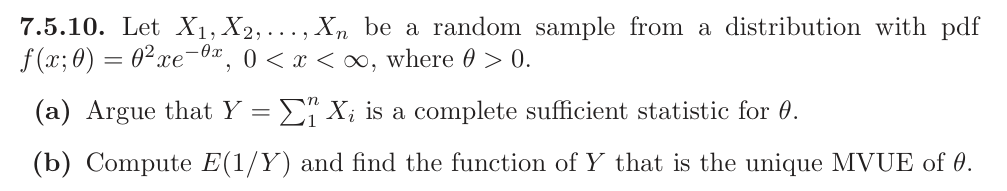
\includegraphics[width=\textwidth]{6-hw12-2025052716.png}
% \caption{}
\label{}
\end{figure}
\end{exercise}
(a)
\[
X_i\sim \Gamma(2,\theta ^{-1})
\]
\[
Y\sim \Gamma(2n,\theta ^{-1})
\]
\[
\frac{\prod_{i=1}^{n} f(x_i;\theta)}{f_{Y}\left( \sum x_i;\theta \right)}=\frac{\theta^{2n}\cdot\left( \prod_{i=1}^{n} x_i \right)\cdot e^{ -\theta \sum x_i }}{\frac{1}{\Gamma(2n)}\theta^{2n}\cdot\left( \sum x_i \right)^{2n-1}e^{ -\theta \sum x_i }}=\frac{\Gamma(2n)\cdot\left( \prod_{i=1}^{n} x_i \right)}{\left( \sum x_i \right)^{2n-1}}
\]
\[
\mathbb{E}(u(Y))=\int_{0}^{\infty} u(y)\cdot\frac{1}{\Gamma(2n)}\theta^{2n}y^{2n-1}e^{ -\theta y } \, \mathrm{d}y=0\implies \int_{0}^{\infty} u(y)y^{2n-1}e^{ -\theta y } \, \mathrm{d}y=0\implies \mathscr{L}(u(y)y^{2n-1})=0
\]
Then
\[
u(y)y^{2n-1}=\mathscr{L}^{-1}(\mathscr{L}(u(y)y^{2n-1})(\theta))=\frac{1}{2\pi i}\int_{\gamma-i\infty}^{\gamma+i\infty} e^{ \theta y }\cdot \underbrace{ \mathscr{L}(u(y)y^{2n-1})(\theta) }_{ =0 } \, \mathrm{d}\theta =0\qquad \forall y\geq 0
\]
Thus $Y$ is complete sufficient statistic.

(b)
\[
\begin{aligned}
E(1/Y) & =\int_{0}^{+\infty} y^{-1}\cdot\frac{1}{\Gamma(2n)}\theta^{2n}y^{2n-1}e^{ -\theta y } \, \mathrm{d}y  \\
 & =\frac{\theta}{\Gamma(2n)} \int_{0}^{+\infty} (\theta y)^{2n-2}e^{ -\theta y } \, \mathrm{d}(\theta y) \\
 & =\frac{\theta}{\Gamma(2n)}\int_{0}^{+\infty} x^{2n-2}e^{ x } \, \mathrm{d}x  \\
 & =\frac{\theta \cdot\Gamma(2n-1)}{\Gamma(2n)} \\
 & =\frac{\theta}{2n-1}
\end{aligned} 
\]
Then $\frac{2n-1}{Y}$ is an unbiased estimator of $\theta$, by Lehmann-Scheffé theorem, $\frac{2n-1}{Y}$ is the unique MVUE of $\theta$.

\begin{exercise}
\begin{figure}[H]
\centering
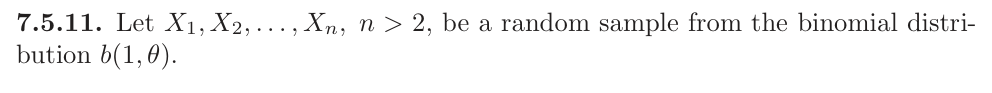
\includegraphics[width=\textwidth]{7-hw12-2025052716.png}
% \caption{}
\label{}
\end{figure}
\begin{figure}[H]
\centering
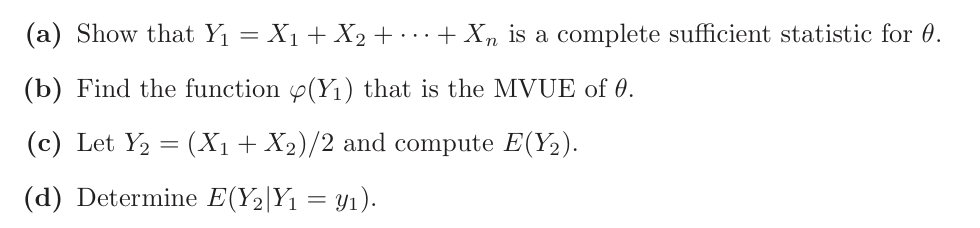
\includegraphics[width=\textwidth]{8-hw12-2025052716.png}
% \caption{}
\label{}
\end{figure}
\end{exercise}
(a) $\theta\in(0,1)$, $Y_1\sim b(n,\theta)$,
\[
\frac{\prod_{i=1}^{n} p(x_i;\theta)}{p_{Y_1}\left( \sum x_i;\theta \right)}=\frac{\theta^{\sum x_i}(1-\theta)^{n-\sum x_i}}{\binom{n}{\sum x_i} \theta^{\sum x_i}(1-\theta)^{n-\sum x_i}}=\frac{1}{\binom{n}{\sum x_i} }
\]
\[
\mathbb{E}[u(Y_1)]=\sum_{k=0}^{n}u(k)\binom{n}{k} \theta^{k}(1-\theta)^{n-k}=0
\]
Let $\theta\to0$, then
\[
0=\sum_{k=0}^{n}u(k)\binom{n}{k} \theta^{k}+O(\theta^{n})\implies u(k)\binom{n}{k} =0,\quad k=0,1,\dots,n-1
\]
Then
\[
0=\sum_{k=0}^{n}u(k)\binom{n}{k} \theta^{k}(1-\theta)^{n-k}=u(n) \theta^{n}\implies u(n)=0
\]
Therefore
\[
u(k)=0\qquad k=0,1,2,\dots,n
\]
$Y_1$ is complete sufficient statistic.

(b)
$\mathbb{E}(Y)=n\theta$, then $\frac{Y}{n}$ is an unbiased estimator of $\theta$; by Lehmann-Scheffé theorem, $\frac{Y}{n}$ is the unique MVUE of $\theta$.

(c)

\begin{table}[h]
	\centering
	\begin{tabular}{|c|c|c|c|}
		\hline
		$Y_2$ & $0$ & $\frac{1}{2}$ & $1$ \\
		\hline
		$P$ & $\theta^{2}$ & $2\theta(1-\theta)$ & $(1-\theta)^2$ \\
		\hline
	\end{tabular}
\end{table}
\[
\begin{aligned}
\mathbb{E}(Y_2) & =0\cdot \mathbb{P}(Y_2=0)+\frac{1}{2}\cdot \mathbb{P}\left( Y_2=\frac{1}{2} \right)+1\cdot \mathbb{P}(Y_2=1) \\
 & =1-\theta
\end{aligned}
\]
(d)
When $y_1\geq2$,
\[
\begin{aligned}
\mathbb{E}(Y_2 \mid Y_1=y_1) & =0\cdot \mathbb{P}(Y_2=0\mid Y_1=y_1)+\frac{1}{2}\cdot \mathbb{P}\left( Y_2=\frac{1}{2}\mid Y_1=y_1 \right)+1\cdot \mathbb{P}(Y_2 =1\mid Y_1=y_1)  \\
 & =\frac{1}{2}\cdot\frac{\mathbb{P}\left( Y_2=\frac{1}{2},Y_1=y_1 \right)}{\mathbb{P}(Y_1=y_1)}+\frac{\mathbb{P}(Y_2=1,Y_1=y_1)}{\mathbb{P}(Y_1=y_1)} \\
 & =\frac{1}{2}\cdot\frac{\mathbb{P}(X_1+X_2=1)\mathbb{P}(X_3+\dots+X_n=y_1-1)}{\mathbb{P}(Y_1=y_1)}+\frac{\mathbb{P}(X_1+X_2=2)\mathbb{P}(X_3+\dots+X_n=y_1-2)}{\mathbb{P}(Y_1=y_1)} \\
 & =\frac{[\binom{n-2}{y_1-2} +\binom{n-2}{y_1-1} ]\theta^{y_1}(1-\theta)^{n-y_1}}{\binom{n}{y_1} \theta^{y_1}(1-\theta)^{n-y_1}} \\
 & =\frac{\binom{n-1}{y_1-1} }{\binom{n}{y_1} } \\
 & =\frac{y_1}{n}
\end{aligned}
\]
And
\[
\begin{aligned}
\mathbb{E}(Y_2\mid Y_1=1) & =0\cdot \mathbb{P}(Y_2=0\mid Y_1=y_1)+\frac{1}{2}\cdot \mathbb{P}\left( Y_2=\frac{1}{2}\mid Y_1=1 \right)+1\cdot \underbrace{ \mathbb{P}(Y_2 =1\mid Y_1=1) }_{ =0 } \\
 & =\frac{1}{2}\cdot\frac{\mathbb{P}(X_1+X_2=1)\mathbb{P}(X_3+\dots+X_n=0)}{\mathbb{P}(Y_1=1)} \\
 & =\frac{\mathbb{P}(X_1+X_2=1)\mathbb{P}(X_3=\dots=X_n=0)}{2\cdot \mathbb{P}(Y_1=1)} \\
 & =\frac{\theta(1-\theta)\cdot\theta^{n-2}}{n\theta^{n-1}(1-\theta)} \\
 & =\frac{1}{n}
\end{aligned}
\]
\[
\mathbb{E}(Y_2 \mid Y_1=1)=0
\]
Thus
\[
\mathbb{E}(Y_2 \mid Y_1=y_1)=\frac{y_1}{n}\qquad y_1=0,1,\dots,n
\]
\begin{exercise}
\begin{figure}[H]
\centering
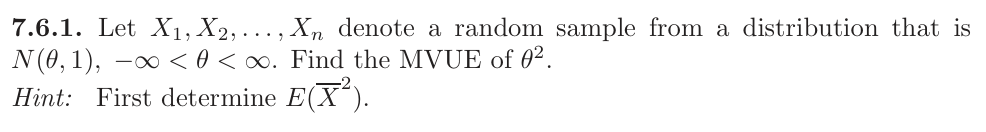
\includegraphics[width=\textwidth]{9-hw12-2025052716.png}
% \caption{}
\label{}
\end{figure}
\end{exercise}
\[
\overline{X}\sim N\left( \theta,\frac{1}{n} \right)
\]
Then
\[
\mathbb{E}(\overline{X}^2)=\int_{-\infty}^{\infty} x^2\cdot\frac{1}{\sqrt{ 2\pi/n  }}\exp \{ -(x-\theta)^2/(2/n ) \} \, \mathrm{d}x =\theta^{2}+\frac{1}{n}
\]
Then $\overline{X}^2-\frac{1}{n}$ is an unbiased estimator of $\theta^{2}$. As $f(x;\theta)=\frac{1}{\sqrt{ 2\pi  }}\exp \{ -(x-\theta)^2/2 \}$, $\frac{1}{n}\sum X_i$ is a complete sufficient statistic for $\theta$. Then $\overline{X}^2-\frac{1}{n}$ is the unique MVUE of $\theta^{2}$.

\begin{exercise}
\begin{figure}[H]
\centering
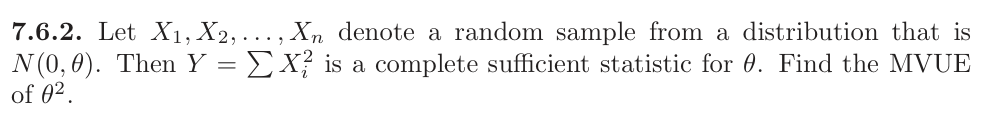
\includegraphics[width=\textwidth]{10-hw12-2025052716.png}
% \caption{}
\label{}
\end{figure}
\end{exercise}
\[
\mathbb{E}Y=\theta^{2}\cdot \mathbb{E}\underbrace{ \left[ \sum\left( \frac{X_i}{\theta} \right)^2 \right] }_{ \sim \chi^{2}(n) }=n\theta^{2}
\]
Then $\mathbb{E}\left[ \frac{Y}{n} \right]=\theta^{2}$. As $Y$ is a complete sufficient statistic for $\theta$, the MVUE of $\theta^{2}$ is $\frac{Y}{n}$.

\begin{exercise}
\begin{figure}[H]
\centering
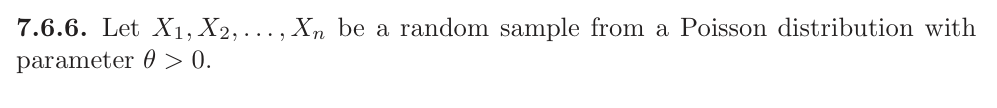
\includegraphics[width=\textwidth]{11-hw12-2025052716.png}
% \caption{}
\label{}
\end{figure}
\begin{figure}[H]
\centering
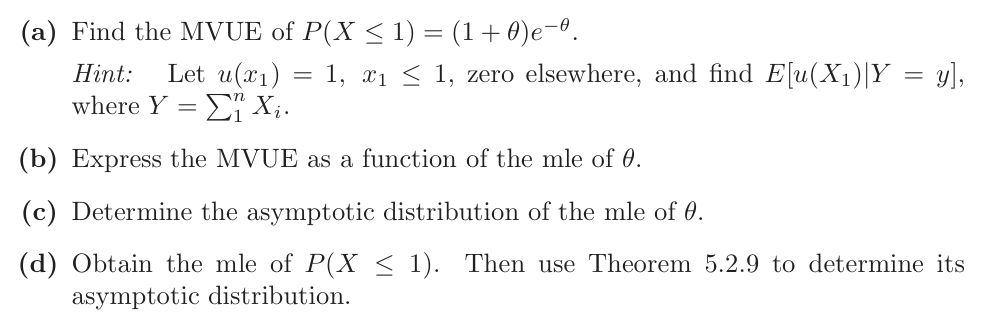
\includegraphics[width=\textwidth]{12-hw12-2025052716.png}
% \caption{}
\label{}
\end{figure}
\end{exercise}
(a)
\[
X_i\sim \text{Poi}(\theta),\quad X_2+\dots+X_n\sim \text{Poi}((n-1)\theta),\quad Y=\sum X_i\sim \text{Poi}(n\theta)
\]
\[
\begin{aligned}
\mathbb{E}[u(X_1)\mid Y=y] & =1\cdot \mathbb{P}(X_1\leq 1 \mid Y=y)+0\cdot \mathbb{P}(X_1>1 \mid Y=y) \\
 & =\mathbb{P}(X_1\leq 1 \mid Y=y) \\
 & =\frac{\mathbb{P}(X_1\leq 1,Y=y)}{\mathbb{P}(Y=y)} \\
 & =\frac{\mathbb{P}(X_1=0)\cdot \mathbb{P}(X_2+\dots+X_n=y)+\mathbb{P}(X_1=1)\cdot \mathbb{P}(X_2+\dots+X_n=y-1)}{\mathbb{P}(Y=y)} \\
 & =\frac{e^{ -\theta }\cdot\frac{1}{y!}[(n-1)\theta]^{y}e^{ -(n-1)\theta }+\theta e^{ -\theta }\cdot\frac{1}{(y-1)!}[(n-1)\theta]^{y-1}e^{ -(n-1)\theta }}{\frac{1}{y!}(n\theta)^{y}e^{ -n\theta }} \\
 & =\left( 1-\frac{1}{n} \right)^{y}+\frac{y}{n}\left( 1-\frac{1}{n} \right)^{y-1}
\end{aligned}
\]
By Lehmann-Scheffé theorem and Rao-Blackwell theorem, $\varphi(Y)\coloneqq \mathbb{E}(u(X_1)\mid Y)$ as an unbiased estimator of $\theta$, is the unique MVUE of $\theta$.
\[
\varphi(Y)=\left( 1-\frac{1}{n} \right)^{Y}+\frac{Y}{n}\left( 1-\frac{1}{n} \right)^{Y-1}
\]
(b)
\[
L(\theta)=\prod_{i=1}^{n} p(x_i;\theta)=\frac{\theta^{\sum x_i}e^{ -n\theta }}{\prod_{i=1}^{n} (x_i!)}
\]
\[
\frac{ \partial   }{ \partial \theta } L(\theta)=\frac{1}{\prod_{i=1}^{n} (x_i!)}\left[ \left( \sum x_i \right)\theta^{\left( \sum x_i \right)-1}e^{ -n\theta }-n\theta^{\sum x_i}e^{ -n\theta } \right]=0\Rightarrow\widehat{\theta}=\frac{1}{n}\sum X_i=\overline{X}
\]
Then the unique MVUE of $\theta$ is
\[
\left( 1-\frac{1}{n} \right)^{n\widehat{\theta}}+\widehat{\theta}\left( 1-\frac{1}{n} \right)^{n\widehat{\theta}-1}
\]
(c)
$\mathbb{E}X_i=\theta,\mathbb{V}X_i=\theta$, by the CLT,
\[
\sqrt{ n }(\overline{X}-\theta)\overset{ \mathcal{D} }{ \to }N(0,\mathbb{V}(X_i))
\]
So
\[
\sqrt{ n }(\widehat{\theta}-\theta)\overset{ \mathcal{D} }{ \to }N(0,\theta)
\]
Thus
\[
\widehat{\theta}\sim N\left( \theta,\frac{\theta}{n} \right)\qquad \text{as }n\to \infty
\]
Whats wrong?:
\[
\varphi_{X_j}(t)=\mathbb{E}(\exp \{ itX_j \})=\sum_{k=0}^{\infty} e^{ itk }\cdot\frac{\theta^{k}e^{ -\theta }}{k!}=\sum_{k=0}^{\infty} \frac{1}{k!}(\theta e^{ it })^{k}e^{ -\theta }=\exp \{ \theta(e^{ it }-1) \}
\]
\[
\begin{aligned}
\varphi_{\widehat{\theta}}(t) & =\mathbb{E}(\exp \{ it\widehat{\theta} \}) \\
 & =\mathbb{E}\left( \exp \left\{  i\frac{t}{n}\sum X_j  \right\} \right) \\
 & =\prod_{j=1}^{n} \mathbb{E}\left( \exp \left\{  i\frac{t}{n}X_j  \right\} \right) \\
 & =\prod_{j=1}^{n}\varphi_{X_j}\left( \frac{t}{n} \right)  \\
 & =\exp \{ n\theta(e^{ it/n  }-1) \} \\
 & =\exp \left\{  n\theta\left( \frac{it}{n}+o(n^{-1}) \right)  \right\} \\
 & =\exp \{ it\theta+o(1) \} \\
 & \to \exp \{ it\theta \}
\end{aligned}
\]
\[
p_{\widehat{\theta}}(x)\to\frac{1}{2\pi}\int_{\mathbb{R}}^{} e^{ it\theta }e^{ -itx } \, \mathrm{d}t=\delta_{\theta} 
\]
(d)
The mle of $\mathbb{P}(X\leq1)=(\theta+1)e^{ -\theta }$ is
\[
(\widehat{\theta}+1)e^{ -\widehat{\theta} }\eqqcolon g(\widehat{\theta})
\]
By theorem 5.2.9,
\[
\sqrt{ n }(g(\overline{X})-g(\theta))\overset{ \mathcal{D} }{ \to }N(0,\theta(g'(\theta))^2)=N(0,\theta^{3}e^{ -2\theta })
\]
Thus
\[
g(\widehat{\theta})\sim N\left( g(\theta),\frac{1}{n}\theta^{3}e^{ -2\theta } \right)\qquad \text{as }n\to \infty
\]
\begin{exercise}
\begin{figure}[H]
\centering
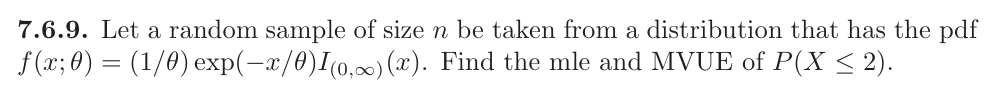
\includegraphics[width=\textwidth]{13-hw12-2025052716.png}
% \caption{}
\label{}
\end{figure}
\end{exercise}
\[
\ell(\theta)=\sum_{i=1}^{n} \log\left( \frac{1}{\theta}e^{ -x_i/\theta } \right)=-\frac{1}{\theta}\sum_{i=1}^{n} x_i-n\log\theta
\]
\[
\frac{ \partial  \ell(\theta) }{ \partial \theta } =\frac{1}{\theta^{2}}\sum_{i=1}^{n} x_i-\frac{n}{\theta}=0\Rightarrow\widehat{\theta}=\frac{1}{n}\sum_{i=1}^{n} X_i=\overline{X}
\]
\[
\mathbb{P}(X\leq 2)=\int_{0}^{2} \frac{1}{\theta}\exp \left\{  -\frac{x}{\theta}  \right\} \, \mathrm{d}x =1-e^{ -2\theta ^{-1} }
\]
MLE:
\[
1-e^{ -2/\widehat{\theta} }=1-\exp \left\{  \frac{2n}{\sum_{i=1}^{n} X_i}  \right\}
\]
\[
f_{X_1\mid Y}(x\mid y)=\frac{f_{X_1,Y}(x,y)}{f_{Y}(y)}
\]
Let
\[
Z\coloneqq X_2+\dots+X_n\sim \Gamma(n-1,\theta)\qquad Y\coloneqq X_1+\dots+X_n\sim \Gamma(n,\theta)
\]
\[
\begin{aligned}
f_{X_1,Y}(x,y) & =f_{X_1,Z}(x,y-x)\begin{vmatrix}
1 & 0 \\
-1 & 1
\end{vmatrix} \\
 & =\frac{1}{\theta}\exp \left\{  -\frac{x}{\theta}  \right\}\cdot\frac{1}{\Gamma(n-1)}\frac{1}{\theta^{n-1}}(y-x)^{n-2}\exp \{ -(y-x)/\theta \} \\
 & =\frac{1}{\theta^{n}}\frac{1}{\Gamma(n-1)}(y-x)^{n-2}\exp \left\{  -\frac{y}{\theta}  \right\}
\end{aligned}
\]
\[
f_{Y}(y)=\frac{1}{\theta^{n}}\frac{1}{\Gamma(n)}y^{n-1}\exp \left\{  -\frac{y}{\theta}  \right\}
\]
\[
f_{X_1\mid Y}(x\mid y)=\frac{f_{X_1,Y}(x,y)}{f_{Y}(y)}=\frac{\frac{1}{\theta^{n}}\frac{1}{\Gamma(n-1)}(y-x)^{n-2}\exp \left\{  -\frac{y}{\theta}  \right\}}{\frac{1}{\theta^{n}}\frac{1}{\Gamma(n)}y^{n-1}\exp \left\{  -\frac{y}{\theta}  \right\}}=(n-1)(y-x)^{n-2}\cdot y^{1-n}
\]
Let
\[
u(x)=\begin{cases}
1 & x\leq 2 \\
0 & x>2 
\end{cases}
\]
For $y\leq2$,
\[
\mathbb{E}(u(X_1)\mid Y=y)=1
\]
For $y>2$,
\[
\mathbb{E}(u(X_1)\mid Y=y)=\int_{0}^{2} u(x)f_{X_1 \mid Y}(x\mid y) \, \mathrm{d}x =\int_{0}^{2} (n-1)(y-x)^{n-2}y^{1-n} \, \mathrm{d}x =1-\left( 1-\frac{2}{y} \right)^{n-1}
\]
$u(X_1)$ is an unbiased estimator of $\mathbb{P}(X\leq2)$. By Lehmann-Scheffé theorem, $\varphi(Y)=\mathbb{E}(u(X_1)\mid Y)$ is the unique MVUE of $\theta$, i.e.
\[
\varphi\left( \sum_{i=1}^{n} X_i \right)=\begin{cases}
1 & \text{if }\sum_{i=1}^{n} X_i\leq 2 \\
1-\left( 1-\frac{2}{\sum_{i=1}^{n} X_i} \right)^{n-1} & \text{if }\sum_{i=1}^{n} X_i>2
\end{cases}
\]